\clearpage
\section{Joint Unknown-Space Exploration Diagnostic}\label{joint-exploration}

Unknown-space exploration remains the broader system objective. A separate 24-trajectory diagnostic starts from a simulated RGB-D/scan packet at 61.50\% reachable-cell coverage, using exact poses and a 0.2 m grid/radius. It compares original V10.3.1 G/S, exploration\_joint\_v1 C/G/S and a local observed-frontier implementation at 48/96-action limits in two related arrangements of one Q0 scene. The joint variant restricts coverage gain to unknown support, diversifies candidates and replans invalidated macro-actions. These declared policy changes distinguish it from the supplied-graph mechanism. All runs return without simulated collision; east/96 C uses 94 actions and the others exhaust their limits. Supplementary Tables S1--S2 retain every outcome.

Three of four G/S conditions tie within each version. In west/96, original S recovers less new reference-visible surface than G (111.44/114.11 m$^2$), while joint S recovers more (118.52/109.51 m$^2$). Joint G/S reach 90/95/99\% coverage at identical actions 18/24/29, with surface histories diverging after 99.55\% coverage. At budget 48, frontier reaches 95\% coverage earlier and gains more observed area, while joint C/G/S recover more surface. The frontier adapter permanently returns after rejection, unlike NSO replanning; common execution protection does not imply equivalent policy contracts.

A post-hoc doubled geometric-prior control exactly reproduces the improved S trajectory in a related two-room case. A separate paid-41 west/96 intervention isolates a ranking unavailable to uniform nonnegative prior reweighting on that saved set, yet gains surface and loses terminal F1 against G. A further synthetic parent fixed before execution yields 11.72 m$^2$ more new surface and 0.04856 higher F1 for S than G/X over complete 96-action routes, but all saved S decisions admit a common geometric-prior weight (supplementary Table S3). These related diagnostics establish conditional allocation effects, with general early-coverage efficiency and category-specific attribution unresolved.

\paragraph{Four-room development pilot.}
A new $16\times12$ m constructed four-room layout contains 16 objects and 121.48 m$^2$ of start-reachable free space. The frozen joint-exploration implementation starts from one rendered RGB-D/scan packet, with no movement prefix and 8.53\% initial coverage. The original 96-action budget and return contract are retained. Inputs include exact simulated odometry and ideal visible semantic labels; an explicit class-2/class-3 dictionary adapter reconciles the older scene generator with the v10 scorer. Hidden geometry is reserved for simulation and evaluation.

Both G and S execute 96 actions, travel 17.2 m, make ten turns, avoid simulated collisions and return to the start. Their coverage curves coincide and reach 39.84\%; neither reaches 90\% coverage. Actions first diverge at step 79, so equal coverage does not imply identical trajectories. This is one development layout with two paired runs, not a completed full-coverage benchmark or an observed semantic efficiency gain. The mapper's surface-patch counts do not measure reconstruction accuracy; the following extension evaluates TSDF quality against a separate exterior reference.

\begin{figure}[!htbp]
\centering
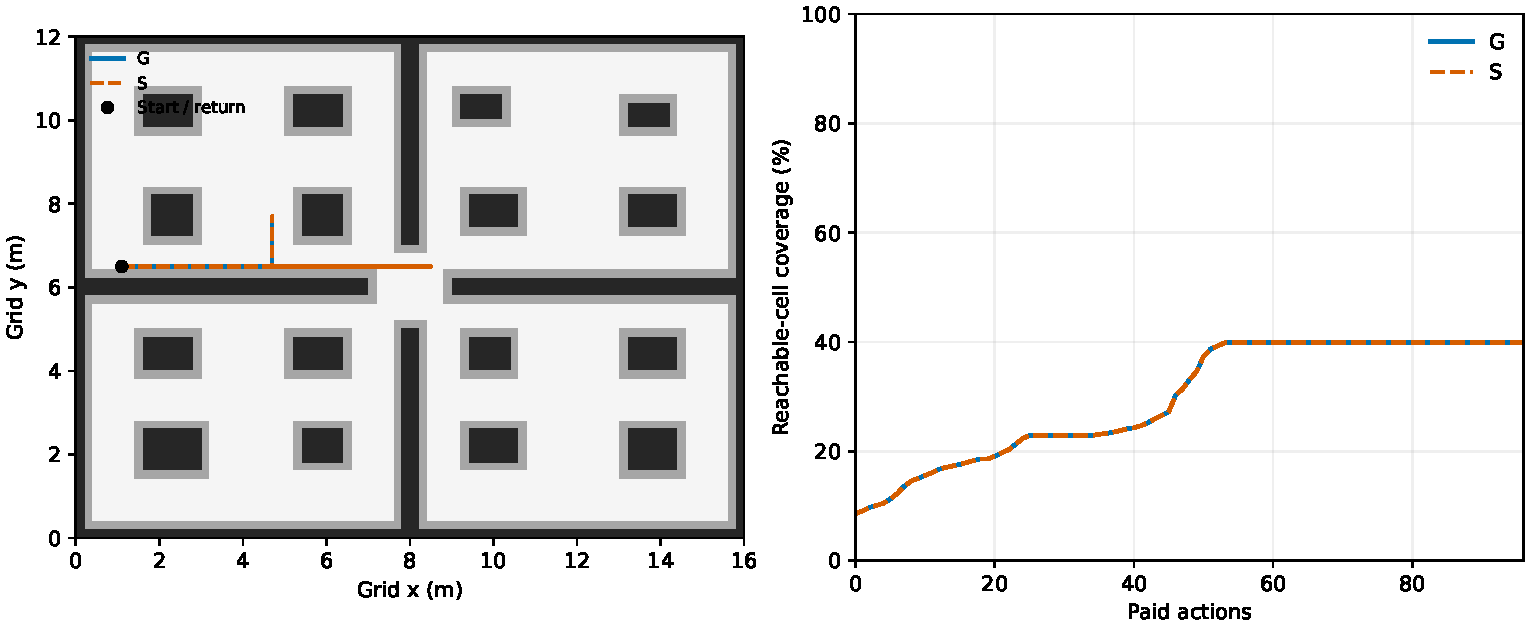
\includegraphics[width=\linewidth]{Unknown_rooms_20261119.pdf}
\caption{Four-room development pilot. Left: evaluator-only occupancy geometry and actual G/S trajectories; the full geometry is not supplied to the planner. Right: coverage measured on the same start-reachable free-cell reference after each paid action. The curves overlap from 8.53\% to 39.84\%, despite a late action difference. Both routes exhaust the 96-action budget and return.}\label{fig:nov19-unknown}
\end{figure}

\paragraph{Budget sufficiency and fixed-cost comparison.}

The development pilot is extended without changing its candidates, scores or execution rules. G attains 85.18\%, 93.38\% and 100\% coverage at budgets 256, 512 and 1024, respectively (Figure~\ref{fig:four-room-budget}). It first covers all free cells in the start-reachable reference at action 727 after 135.0 m; the complete 1024-action episode travels 189.6 m and returns without collision or false occupied labels on that reference. These are one-layout budget diagnostics. A matched S/1024 attempt receives SIGTERM after 398 actions and 93.38\% last-observed coverage; its cause is undetermined, and no terminal outcome or policy failure is assigned.

\begin{figure}[!htbp]\centering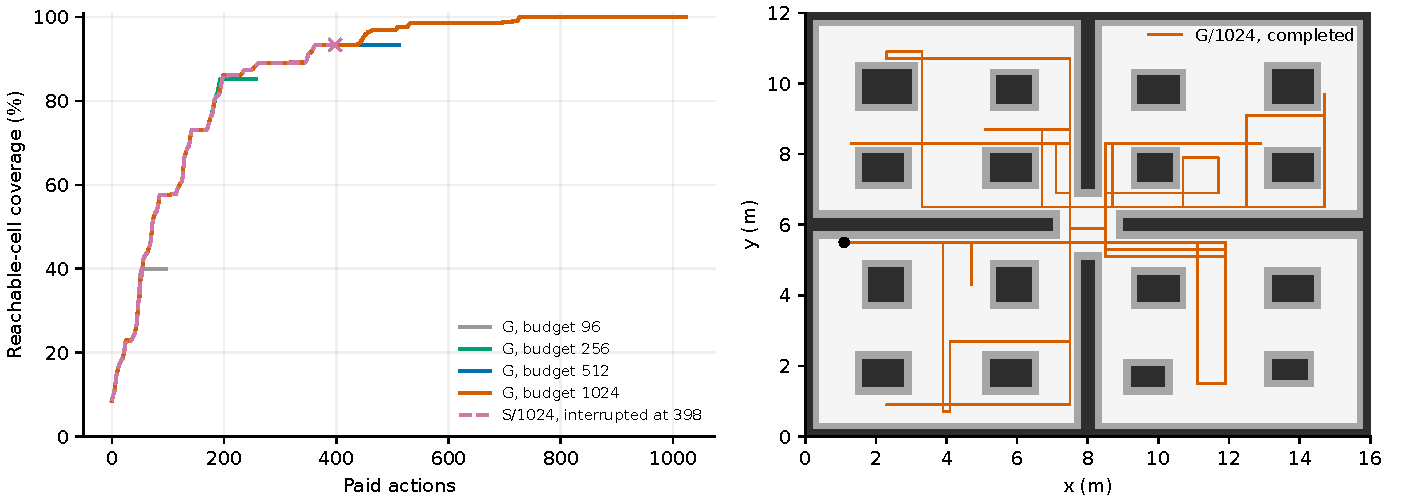
\includegraphics[width=.94\linewidth]{Four_room_budget_20261119.pdf}

\caption{Development budget diagnostics, retaining the shorter incomplete trials. The interrupted S curve ends at its last actual observation. Right: the completed G/1024 trajectory over evaluator-only geometry. Full coverage is a measured checkpoint, separate from the later return.}\label{fig:four-room-budget}\end{figure}

A separate frozen protocol compares six arms at a common 512-action cap on three generated object layouts: the inspected development layout D and two new layouts E1/E2, all sharing one four-room wall topology. Each paired set begins with an identical single sensor packet and exact pose. C scores unknown coverage; G adds measured quality and a generic structural prior; S uses category-conditioned priors; X reverses that interpretation. G2 doubles only the generic prior. S with frozen gain disables only the radar/camera posterior update while retaining fusion and directional histories. All eighteen runs are retained (Table~\ref{tab:four-room-matrix}); they represent three layouts, not eighteen independent environments.

The renderer supplies constant-gray valid RGB pixels and ideal visible category labels. Objects occupy regularly arranged slots, with no natural-image detector or measured real-world category distribution. These scenes test a synthetic planning mechanism, not realistic semantic perception. Neither the complete two-template posterior nor a trained reachability network runs in this joint variant.

Native measured-depth TSDF meshes use 6 cm voxels and 12 cm truncation. A fixed reference samples the exterior box-union boundary, excluding internal faces, and retains surfaces visible from a 0.8 m lattice of reachable camera origins. Reconstructed-area precision and fixed-reference recall at 5 cm yield surface F1~\cite{ref14}. The reference is independent of each trajectory; the supplementary protocol specifies its sampling and visibility limits.

\begin{table}[!htbp]\centering\small

\caption{All eighteen outcomes at a common 512-action cap. Entries are reachable-cell coverage / surface F1 at 5 cm, both in percent. D is development; E1/E2 are new object layouts of the same topology.}\label{tab:four-room-matrix}

\begin{tabular}{@{}lrrr@{}}\toprule Policy & D: Coverage/F1 & E1: Coverage/F1 & E2: Coverage/F1 \\ \midrule

C & 97.43/94.73 & 98.08/93.59 & 98.03/93.53 \\

G & 93.38/89.36 & 94.59/93.28 & 94.67/87.68 \\

S & 93.38/89.36 & 94.59/93.19 & 94.67/87.68 \\

X (reversed cue) & 93.91/90.09 & 94.86/93.71 & 98.03/93.13 \\

G, $2\times$ prior & 93.38/89.36 & 94.59/93.28 & 94.67/87.68 \\

S, frozen gain & 93.38/90.17 & 94.59/93.19 & 94.67/87.68 \\

\bottomrule\end{tabular}\end{table}

C exceeds G and S in both coverage and F1 on all three layouts; X also exceeds S in F1 throughout. G/S trajectories coincide in D/E2. In E1 they differ but finish with equal coverage, while S lowers F1 by 0.083 percentage points; its normalized coverage-curve area increases by only 0.000968. G2 reproduces G in all three layouts. Freezing the gain posterior improves F1 only in D, with unchanged coverage. These outcomes provide no consistent benefit from the semantic prior or gain calibration.

A post-hoc audit nevertheless distinguishes ranking from utility. For E1, four recorded S choices cannot be reproduced by any nonnegative weight in $\mathrm{common}+\lambda\,\mathrm{prior}_G$, even separately at each state, with the original cost/id tie rule. D/E2 admit uniform weights including 1 and 2. Category-conditioned ranking therefore operates in E1 without an observed endpoint benefit. On D, replay of the 98-action zero-coverage segment raises surface F1 from 88.185\% to 88.930\%: observation is useful locally but inefficient relative to the coverage control. Detailed score intervals, reference construction and replay results are retained in the supplement.

\begin{figure}[H]\centering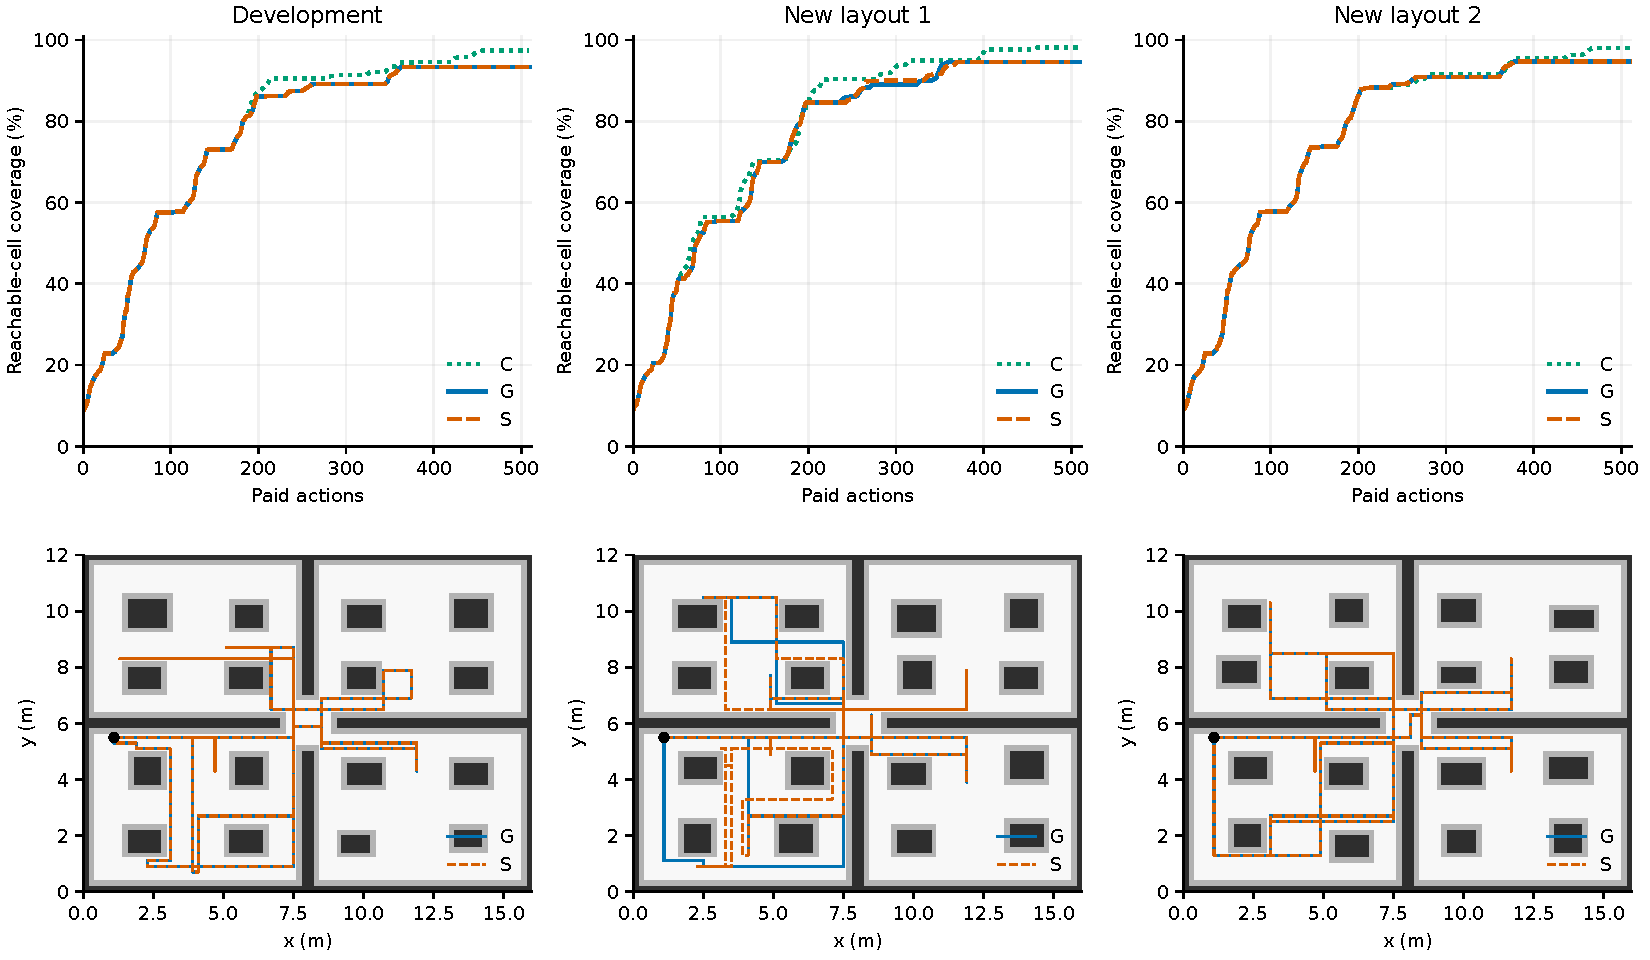
\includegraphics[width=.94\linewidth]{Four_room_matrix_20261119.pdf}

\caption{Fixed-cost coverage histories and G/S trajectories for D/E1/E2. Background geometry is evaluator-only. The full table retains the additional controls; repeated checkpoints are dependent measurements.}\label{fig:four-room-matrix}\end{figure}


A further diagnostic uses the original textured ReplicaCAD apartment layout with partial oracle labels and the unchanged observed-state joint policy (supplementary Table~S7). Coverage-only C reaches 100.00\% coverage and 92.32\% surface F1 within the common 256-action cap; G/S and both label controls yield identical trajectories, 95.62\% coverage and 90.28\% F1. The original grouping stage rejects the oversized components containing semantic observations before class-dependent scoring. This single-layout transfer test remains separate from the V35 controlled study and does not establish natural-detector or physical performance.

A further controlled extension replaces that analytic prior with the V3 box/shelf expected visible-area module while retaining v10 unknown coverage, measured quality, candidates, and return rules. Twelve runs compare six arms in two furniture permutations of one synthetic branching layout, using original textured assets and partial ideal semantics (supplementary Table~S8). All runs reach full reference coverage and return without simulated collision. G/S produce identical trajectories; the joint control without templates ties them in one layout and exceeds their surface F1 by 0.36 percentage points in the other at the same 256-action budget. C reaches full coverage sooner and ends after 130 actions. The extension establishes complete exploration in these controlled layouts, without a semantic or completion-module efficiency advantage. Fixed-action replay then reproduces its measurements, saved scores, and final TSDF exactly. It identifies a visibility inconsistency: a template surface contradicted by acquired free space can still occlude other hypothetical surfaces. A separately frozen repair preserves measured and unknown occluders while skipping strictly free intersections. Across another twelve paired runs on the same layouts, it raises left-layout G/S F1 from 92.40\% to 92.63\%, still below J at 92.76\%; the right layout is unchanged. G/S remain trajectory-identical, and their first full-coverage actions are unchanged. Same-point prediction checks recover some subsequently reconstructed surface support but retain substantial template mismatch (supplementary Tables~S9--S10 and the paired-change figure). Thus neither revision establishes a semantic advantage in unknown exploration.

Fixed-prefix diagnostics isolate template sampling, geometry, free-space evidence and object support on the same six acquired states and 66 outbound branches. The earlier geometry/pooling variants retain substantial prediction mismatch and no semantic efficiency benefit (supplementary Table~S11). A clean six-run full-basis ablation shows that measured-surface consumption can improve F1 while delaying full coverage (Table~S12). A further declared revision O constructs completion hypotheses only for acquired positive instance tracks; measured mapping, unknown coverage and candidates are unchanged. G and S share the ideal instance frontend, so G is a neutral structural-class control rather than a completely semantics-free system. Outer-plane and layer-placement revisions improve some prediction components but do not exceed O in realized surface prediction and ranking (supplementary Table~S13); they are not promoted as stand-alone policy revisions. Fixed acquired-ray depth profiles prefer smaller depths but cannot exclude the 0.65~m prior under their predeclared heuristic band, so that profile applies no dimension update.

All eight O-policy runs complete coverage, return and record zero simulated collisions (supplementary Table~S14). On the left, S reaches full coverage at action 97 versus 88 for G, travels 1.2~m farther, and loses 0.377 percentage points of 5~cm F1. Shelf recall rises by 1.294 points while cabinet recall falls by 2.834 points. G/S remain trajectory- and mesh-identical on the right. Removing only the inherited geometric likelihood leaves both S trajectories unchanged; removing only measured-surface consumption yields mixed outcomes. The first changed left-layout decision is driven mainly by a misplaced cabinet hypothesis, illustrating how a category prior can amplify geometry error. These results establish controlled exploration feasibility and a semantic decision effect, without a semantic efficiency advantage.

A separately frozen revision represents unresolved depth and unseen-extent placement with joint structure--geometry particles. It replaces the earlier surface-only update with one loss-based observation update \cite{bissiri2016}; G/S share the acquired support and geometric errors. An independent set of 24 procedural objects is split by object into 12 training, six validation and six held-out objects. Training CRPS selects 0.01~m, the lower endpoint of eight declared scales. On the predeclared front--side/around-object subset, validation/held-out CRPS is 0.0213/0.0229~m versus 0.1761/0.1570~m for the conditioned prior. All seven unusable cases remain in full-denominator evaluation. Nominal 95\% intervals cover only 9/12 and 8/12 subset cases; the result is not nominal probability calibration \cite{syring2019}. Supplementary Tables~S15--S16 and the four-condition figure retain the front-view weakness, failure cases and interval widths.

Ten complete runs compare matched G/S fixed, G/S distribution and S posterior-mean policies with unchanged 256-action budgets. All reach 100\% correct-free coverage, return and incur zero simulated collisions (supplementary Table~S18). On the left, distribution and mean modes reach full coverage at action 88 rather than 97, shorten travel from 43.2 to 42.0~m and raise 5~cm F1 from 92.381\% to 92.758\%; cabinet recall rises by 2.834 percentage points while shelf recall falls by 1.294 points. All right-layout outcomes tie. Within both extent modes, G/S trajectories and measured meshes are identical; mean collapse also reproduces the full distribution in both layouts. Category priors change some scores but never the selected candidate. The six-state forecast comparison (Table~S17) likewise favors mean collapse over distribution in aggregate realized weight and rank. Thus this revision supports a benefit from replacing fixed extent in one inspected layout, without a demonstrated semantic or distribution-spread advantage. Distribution computation is also more expensive. These simulated timings are not robot control measurements.

